\documentclass[UTF8]{ctexart}
\usepackage{geometry}
\usepackage[backend=biber, style=authoryear]{biblatex} % 示例配置
\addbibresource{references.bib} % 替换为你的参考文献文件
\geometry{margin=1.5cm, vmargin={0pt,1cm}}
\setlength{\topmargin}{-1cm}
\setlength{\paperheight}{29.7cm}
\setlength{\textheight}{25.3cm}

% useful packages.
\usepackage{amsfonts}
\usepackage{amsmath}
\usepackage{amssymb}
\usepackage{amsthm}
\usepackage{enumerate}
\usepackage{graphicx}
\usepackage{multicol}
\usepackage{fancyhdr}
\usepackage{layout}
\usepackage{listings}
\usepackage{xcolor}
\usepackage{multirow}
\lstset{language=C++}
\setlength{\headheight}{13pt}  % 增加头部高度
\usepackage{float, caption}

% Listings setting for code formatting
\lstset{
    basicstyle=\ttfamily,
    keywordstyle=\color{blue},
    commentstyle=\color{gray},
    stringstyle=\color{red},
    breaklines=true,
    frame=single,
    numbers=left,
    numberstyle=\tiny,
    stepnumber=1,
    tabsize=4
}

% some common commands
\newcommand{\dif}{\mathrm{d}}
\newcommand{\avg}[1]{\left\langle #1 \right\rangle}
\newcommand{\difFrac}[2]{\frac{\dif #1}{\dif #2}}
\newcommand{\pdfFrac}[2]{\frac{\partial #1}{\partial #2}}
\newcommand{\OFL}{\mathrm{OFL}}
\newcommand{\UFL}{\mathrm{UFL}}
\newcommand{\fl}{\mathrm{fl}}
\newcommand{\op}{\odot}
\newcommand{\Eabs}{E_{\mathrm{abs}}}
\newcommand{\Erel}{E_{\mathrm{rel}}}

\begin{document}

\pagestyle{fancy}
\fancyhead{}
\lhead{陈梓锐}
\chead{22435036}
\rhead{\today}


%\begin{abstract}
 %   The abstract is not necessary for the theoretical homework, 
   % but for the programming project, 
    %you are encouraged to write one.      
%\end{abstract}

% ============================================
\section*{理论作业}
\subsection*{Exercise 12.42}
只需证明对$\forall U \in L^1(h\mathbb{Z} )$,傅里叶 + 逆 = 恒等变换.

即$U(m) = \frac{1}{\sqrt{2\pi}} \int_{-\frac{\pi}{h}}^{\frac{\pi}{h}} e^{imh\xi}\hat{U}(\xi) \dif\xi$

因为$U\in L^1(h\mathbb{z}) \Rightarrow \sum_{m\in\mathbb{Z}} |U(m)| < \infty$

又因为$\forall m\in \mathbb{z}, \forall \xi \in[-\frac{\pi}{h}, \frac{\pi}{h}], |e^{-imh\xi}|\leq |U_m|$.

因此，$\forall \xi\in [-\frac{\pi}{h}, \frac{\pi}{h}], \frac{1}{\sqrt{2\pi}}\sum_{m\in\mathbb{z}}|e^{-imh\xi}U_mh| \leq \frac{1}{\sqrt{2\pi}}\sum_{m\in\mathbb{z}}|U_m|h \leq \infty$

所以$\hat{U}(\xi) = \frac{1}{\sqrt{2\pi}}\sum_{m\in\mathbb{z}} e^{-imh\xi}U_mh$在$\xi \in [-\frac{\pi}{h}, \frac{\pi}{h}]$上一致收敛，
则求和和积分可换序。
\begin{equation}
    \label{eq:12.42}
    \begin{aligned}
        \hat{U}(\xi) &= \frac{1}{\sqrt{2\pi}}\sum_{m\in\mathbb{z}} e^{-imh\xi}U(m)h \\
                     &= \frac{1}{\sqrt{2\pi}}\int_{-\frac{\pi}{h}}^{\frac{\pi}{h}} (\frac{1}{\sqrt{2\pi}}e^{inh\xi}\sum_{n\in\mathbb{z}} e^{-imh\xi}U(n)h )\dif\xi \\
                     &= \frac{1}{2\pi}\sum_{n\in \mathbb{z}}\int_{-\frac{\pi}{h}}^{\frac{\pi}{h}} e^{i(m-n)h\xi}U(n)h \dif\xi 
    \end{aligned}    
\end{equation}
因为$\begin{aligned}
    \int_{-\frac{\pi}{h}}^{\frac{\pi}{h}} e^{i(m-n)h\xi} \dif\xi = 
        \begin{cases}
            \dfrac{2\pi}{h} & \text{if } m = n, \\
            0 & \text{otherwise.}
        \end{cases}
\end{aligned}$,

代入式\eqref{eq:12.42}得证.

\subsection*{Exercise 12.49}
$\theta method :$

$-\theta rU^{n+1}_{i-1} + (1+2\theta r)U_i^{n+1} - \theta rU^{n+1}_{i} = (1-\theta)rU^n_{i-1} + (1 - 2(1-\theta)r)U^n_i + (1-\theta)rU^n_{i+1}$

使用fourier变换：
\begin{equation}
    \label{eq:12.49}
    \begin{aligned}
        U_j^{n+1} &= \frac{1}{\sqrt{2\pi}}\int_{-\frac{\pi}{h}}^{\frac{\pi}{h}} 
        (-\theta re^{i(j-1)h\xi} + (1+2\theta r)e^{ijh\xi} - \theta re^{i(j+1)h\xi} )\hat{U}{n+1}_j(\xi) \dif\xi \\
        &= \frac{1}{\sqrt{2\pi}}\int_{-\frac{\pi}{h}}^{\frac{\pi}{h}}
        ((1-\theta)re^{i(j-1)h\xi} + (1 - 2(1-\theta)r)e^{ijh\xi} + (1-\theta)re^{i(j+1)h\xi} )\hat{U}^{n}_j(\xi) \dif\xi 
    \end{aligned}
\end{equation}

\eqref{eq:12.49}两边同除$e^{ijh\xi}$可得： 

$(-\theta re^{-ih\xi} + (1+2\theta r) - \theta re^{ih\xi})\hat{U}^{n+1}(\xi) = ((1-\theta)re^{-ih\xi} + (1 - 2(1-\theta)r) + (1-\theta)re^{ih\xi})\hat{U}^{n}(\xi)$

即
\begin{equation}
    \label{eq:12.49-2}
    \begin{aligned}
        \hat{U}^{n+1}(\xi) &= \frac{1-4(1-\theta)r\sin^2(\frac{h\xi}{2})}{1+4\theta r\sin^2(\frac{h\xi}{2})}\hat{U}^{n}(\xi) 
    \end{aligned}
\end{equation}
要使$|\frac{1-4(1-\theta)r\sin^2(\frac{h\xi}{2})}{1+4\theta r\sin^2(\frac{h\xi}{2})}| < 1$，需要$\forall\xi\in[-\frac{\pi}{h}, \frac{\pi}{h}]$
\begin{equation}
    \label{eq:12.49-3}
    \begin{aligned}
        -(1-\theta)\sin^2(\frac{h\xi}{2}) < \theta \sin^2(\frac{h\xi}{2})
    \end{aligned}
\end{equation}
\begin{equation}
    \label{eq:12.49-4}
    \begin{aligned}
        2(1-2\theta)r\sin^2(\frac{h\xi}{2}) \leq 1
    \end{aligned}
\end{equation}

因为$\theta\in [0,1]$，所以\eqref{eq:12.49-3}一定成立，考虑\eqref{eq:12.49-4}，

当$\theta \in [\frac{1}{2}, 1]$时，$2(1-2\theta)r\sin^2(\frac{h\xi}{2}) \leq 0 < 1$，

当$\theta \in [0, \frac{1}{2})$时，$2(1-2\theta)r\sin^2(\frac{h\xi}{2}) \leq 2(1-2\theta)r < 1$，.
$r = \frac{kv}{h^2} \Rightarrow < \frac{h^2}{2(1-2\theta)v}$

Fourier变换让我们能从频率的角度来看待问题，将复杂的PDE简化为代数问题。


\subsection*{Exercise 12.78}
$\mu = \frac{ak}{h}$

\begin{equation}
    \label{eq:12.78-1}
    \begin{aligned}
        &(12.89a)： \\
        &\tau(x,t) = u(x, t+k) - u(x,t) + \frac{ak}{2h}(3u(x,t)- 4u(x-h,t) + u(x-2h,t))-\frac{a^2k^2}{2h^2}(u(x,t)-2u(x-h,t)+u(x-2h,t))
    \end{aligned}
\end{equation}
\begin{equation}
    \begin{aligned}
        u(x,t+k) &= u(x,t) + ku_t(x,t) + \frac{k^2}{2}u_{tt}(x,t)+o(k^2) \\
        u(x-h,t) &= u(x,t) - hu_x(x,t) + \frac{h^2}{2}u_{xx}(x,t)-\frac{h^3}{6}u_{xxx}(x,t)+o(h^3) \\
        u(x-2h,t) &= u(x,t) - 2hu_x(x,t) + 2h^2u_{xx}(x,t)-\frac{4h^3}{3}u_{xxx}(x,t)+o(h^3) \\
        u_t &= -au_{xx}
    \end{aligned}
\end{equation}
代入\eqref{eq:12.78-1}可得：
$$\tau(x,t) = -aku_x + \frac{k^2}{2}a^2u_{xx} + \frac{ak}{2h}(2hu_x - \frac{2}{3}h^3u_{xxx} + o(h^3)) -\frac{a^2k^2}{2h^2}(h^2u_{xx} - h^3u_{xxx} + o(h^3)) = o(h^2 + k^2)$$

(12.89b)可类似得到。

\subsection*{Exercise 12.79}
(12.89a)
用Fouier变换：
\begin{equation}
    \label{eq:12.79-1}
    \begin{aligned}
        U^{n+1}_j &= \frac{1}{\sqrt{2\pi}}\int_{-\frac{\pi}{h}}^{\frac{\pi}{h}} 
        [e^{ijh\xi} - \frac{\mu}{2}(3e^{ijh\xi} - 4e^{i(j-1)h\xi} + e^{i(j+1)h\xi}) + \frac{\mu^2}{2}(e^{ijh\xi} - 2e^{i(j-1)h\xi} + e^{i(j+1)h\xi})]\hat{U^n_j}(\xi) \dif\xi \\
        &= \frac{1}{\sqrt{2\pi}}\int_{-\frac{\pi}{h}}^{\frac{\pi}{h}} e^{ih\xi}\hat{U}^{n+1}_j(\xi) \dif\xi 
    \end{aligned}
\end{equation}

如Exercise 12.49可得
\begin{equation}
    \label{eq:12.79-2}
    \begin{aligned}
        \hat{U}^{n+1}(\xi) &= [(1-\frac{3}{2}\mu + \frac{\mu^2}{2}) + (2\mu - \mu^2)e^{-ih\xi} + (\frac{\mu^2-\mu}{2}e^{-2ih\xi})]\hat{U}^n(\xi) \\
                           &= e^{-ih\xi}[(1-2\mu+\mu^2)\cos h\xi + (1-\mu)i\sin h\xi + (2\mu- \mu^2)]\hat{U}^n_j(\xi) \\
                           &= e^{-ih\xi}[(1-2\mu+\mu^2)(-2\sin^2\frac{h\xi}{2})+(1-\mu)i\sin h\xi + 1]\hat{U}^{n}(\xi)
    \end{aligned}
\end{equation}
要使
\begin{equation}
    \label{eq:12.79-3}
    \begin{aligned}
        |e^{-ih\xi}[(1-2\mu+\mu^2)(-2\sin^2\frac{h\xi}{2})+(1-\mu)i\sin h\xi + 1]| &\leq 1 \\
        |(1-2\mu+\mu^2)(-2\sin^2\frac{h\xi}{2})+(1-\mu)i\sin h\xi + 1|^2 &\leq 1 \\
         4\mu(2-\mu)(1-\mu^2)\sin^4(\frac{h\xi}{2}) &\geq 0
    \end{aligned}
\end{equation}
解得$\mu \in[0,2]$.

(12.89b)类似可得。

\begin{figure}[H]
    \centering
    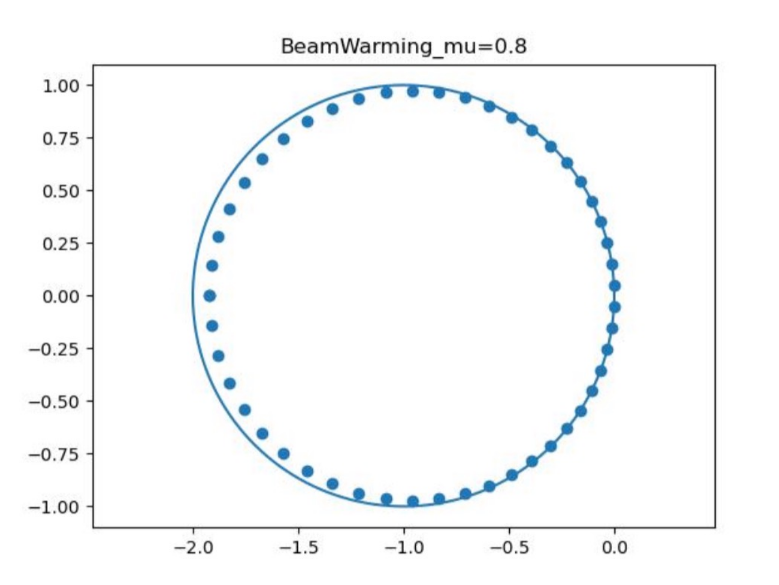
\includegraphics[width=0.2\textwidth]{fig12.79-1.png}
    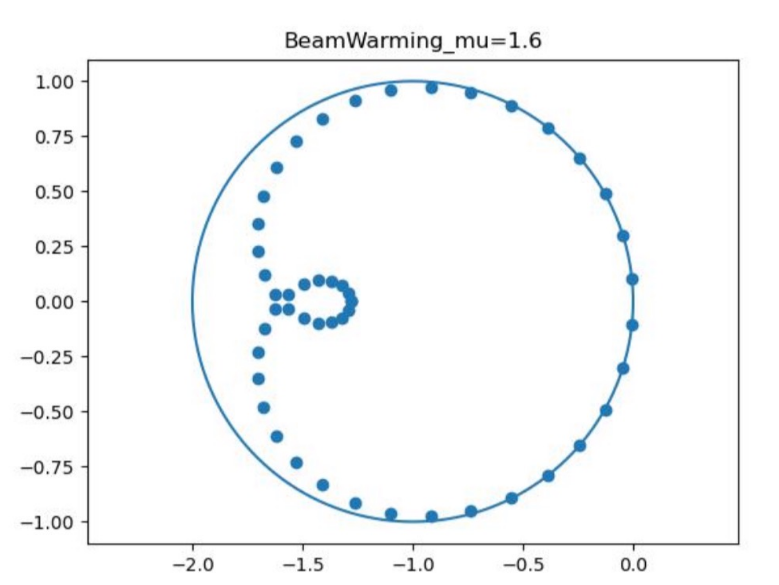
\includegraphics[width=0.2\textwidth]{fig12.79-2.png}
    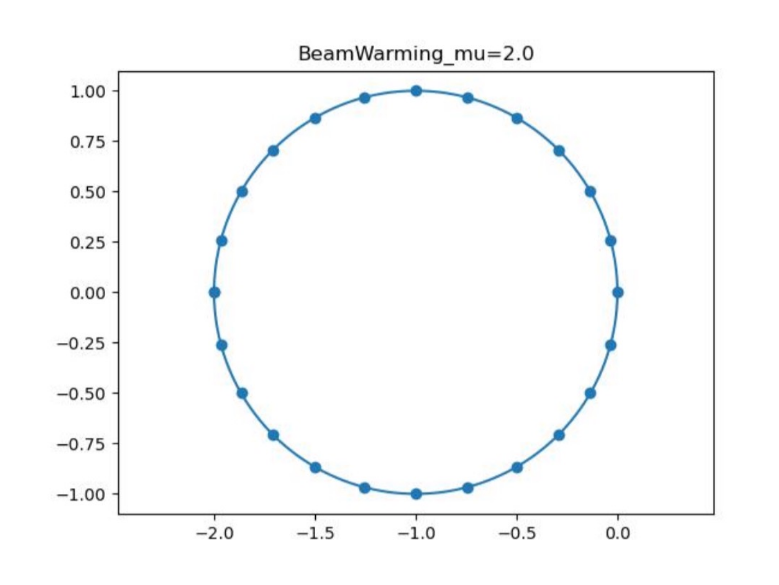
\includegraphics[width=0.2\textwidth]{fig12.79-3.png}
    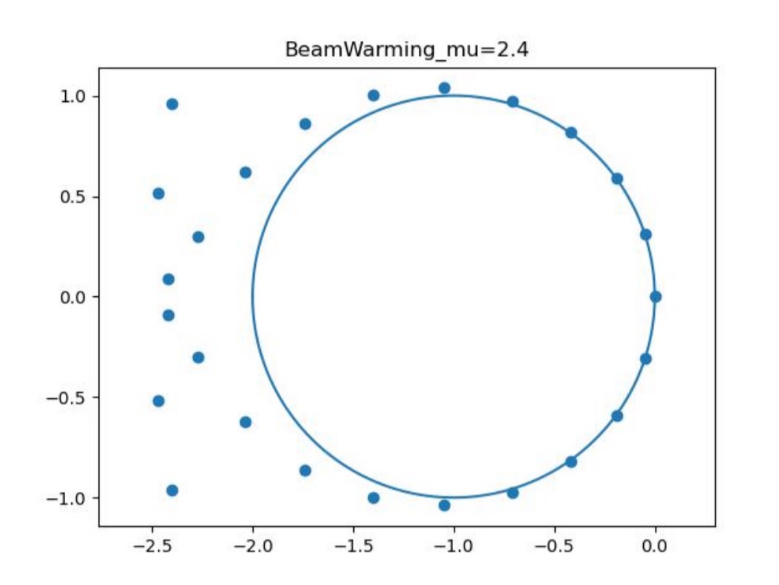
\includegraphics[width=0.2\textwidth]{fig12.79-4.png}
\end{figure}


\subsection*{Exercise 12.82}
\begin{figure}[H]
    \centering
    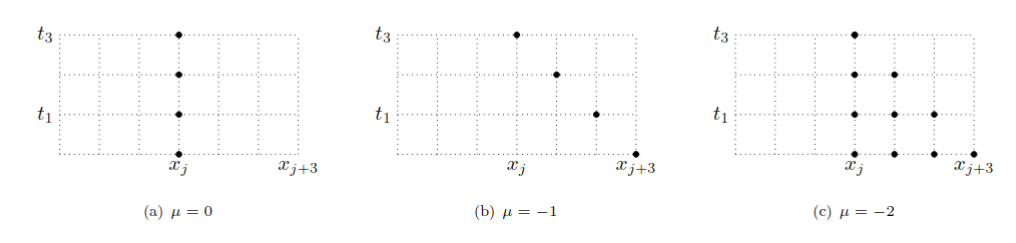
\includegraphics[width=0.7\textwidth]{12.82.png}
\end{figure}

\subsection*{Exercise 12.83}
\begin{figure}[H]
    \centering
    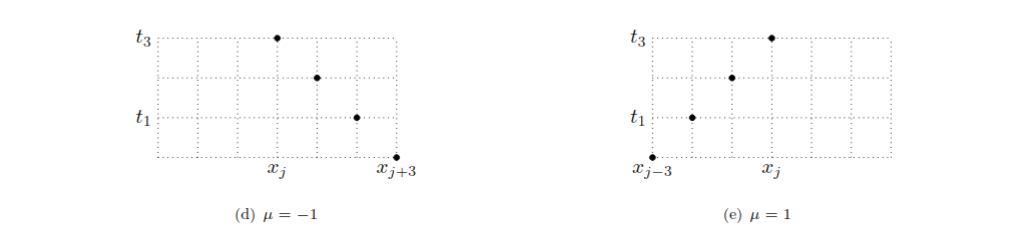
\includegraphics[width=0.5\textwidth]{12.83.png}
\end{figure}



\subsection*{Exercise 12.92}
Leapfrog method:
$\frac{v(x,t+k)-v(x,t-k)}{2k} + a\frac{v(x+h,t) - v(x-h,t)}{2h} = 0,$在(x,t)处taylor展开并且假设h=O(h)，可得
\begin{equation}
    \label{eq:12.92-T}
    \begin{aligned}
        v_t + av_x = -\frac{1}{6}(k^2v_{ttt}+ah^2v_{xxx}) - \frac{1}{120}(k^4v_{ttttt}+ah^4v_{xxxxx}) + O(k^5)
    \end{aligned}
\end{equation}

\eqref{eq:12.92-T}对t求导：
\begin{equation}
    \label{eq:12.92-1}
    \begin{aligned}
        v_{tt} = -av_{xt} - \frac{k^2}{6}v_{tttt} - \frac{ah^2}{6}v_{xxxt} + O(k^3)
    \end{aligned}
\end{equation}

\eqref{eq:12.92-T}对x求导：
\begin{equation}
    \label{eq:12.92-2}
    \begin{aligned}
        v_{xt} = -av_{xx} - \frac{k^2}{6}v_{xttt} - \frac{ah^2}{6}v_{xxxx} + O(k^3)
    \end{aligned}
\end{equation}

\eqref{eq:12.92-2}$\times$a - \eqref{eq:12.92-1}：
\begin{equation}
    \label{eq:12.92-3}
    \begin{aligned}
        v_{tt} = a^2v_{xx} - \frac{k^2}{6}(v_{tttt} - av_{xttt}) - \frac{ah^2}{6}(v_{xxxt} - av_{xxxx}) + O(k^3)
    \end{aligned}
\end{equation}

\eqref{eq:12.92-3}对t求导：
\begin{equation}
    \label{eq:12.92-4}
    \begin{aligned}
        v_{ttt} = a^2v_{xxt} - \frac{k^2}{6}(v_{ttttt}-av_{xtttt}) - \frac{ah^2}{6}(v_{xxxtt}-av_{xxxxt}) + O(k^3)
    \end{aligned}
\end{equation}

\eqref{eq:12.92-2}对x求导：
\begin{equation}
    \label{eq:12.92-5}
    \begin{aligned}
        v_{xxt} = -av_{xxx} -\frac{k^2}{6}v_{xxttt} -\frac{ah^2}{6}v_{xxxxx} + O(k^3)
    \end{aligned}
\end{equation}

\eqref{eq:12.92-5}$\times a^2$ + \eqref{eq:12.92-4}：
\begin{equation}
    \label{eq:12.92-6}
    \begin{aligned}
        v_{ttt} = -a^3v_{xxx} - \frac{k^2}{6}(v_{ttttt} -av_{xtttt}+a^2v_{xxttt})-\frac{ah^2}{6}(v_{xxxtt}-av_{xxxxt}+a^2v_{xxxxx}) + O(k^3)
    \end{aligned}
\end{equation}

\eqref{eq:12.92-2}对x求两次导：
\begin{equation}
    \label{eq:12.92-7}
    \begin{aligned}
        v_{xxxxt} = -av_{xxxxx} + O(k^2)
    \end{aligned}
\end{equation}

\eqref{eq:12.92-1}对x求三次导,代入\eqref{eq:12.92-7}：
\begin{equation}
    \label{eq:12.92-8}
    \begin{aligned}
        v_{xxxtt} = a^2v_{xxxxx} + O(k)
    \end{aligned}
\end{equation}

\eqref{eq:12.92-3}对x求两次导，代入\eqref{eq:12.92-7}：
\begin{equation}
    \label{eq:12.92-9}
    \begin{aligned}
        v_{xxttt} = -a^3v_{xxxxx} + O(k)
    \end{aligned}
\end{equation}

\eqref{eq:12.92-5}对x，t各求一次导，代入\eqref{eq:12.92-8}
\begin{equation}
    \label{eq:12.92-10}
    \begin{aligned}
        v_{xtttt} = a^4v_{xxxxx} + O(k)
    \end{aligned}
\end{equation}

\eqref{eq:12.92-6}对t求两次导，代入\eqref{eq:12.92-8}：
\begin{equation}
    \label{eq:12.92-11}
    \begin{aligned}
        v_{ttttt} = -a^5v_{xxxxx} + O(k)
    \end{aligned}
\end{equation}

将上式代入\eqref{eq:12.92-T}：
\begin{equation}
    \label{eq:12.92-12}
    \begin{aligned}
        &v_t + av_x + \frac{ak^2}{6}(1-\mu^2)v_{xxx}+O(k^3) =\epsilon_fv_{xxxxx} \\
        &v_t + av_x + \frac{ak^2}{6}(1-\mu^2)v_{xxx} = 0
    \end{aligned}
\end{equation}

Lax-Wendroff 同理。




\subsection*{Exercise 12.93}
$u_t = -au_x$
由(12.89a):$\frac{v(x,t+k)-v(x,t)}{k} + a\frac{3v(x,t) - 4v(x-h,t) + v(x-2h,t)}{2h} = ka^2\frac{v(x,t) - 2v(x-h,t) + v(x-2h,t)}{2h^2}.$
\begin{equation}
    \label{eq:12.93-T}
    \begin{aligned}
        v_t + av_{xx} = \frac{k}{2}(a^2v_{xx}-v_{tt})-\frac{k^2}{6}v_{ttt}+(\frac{ah^2}{3}-\frac{kha^2}{2})v_{xxx}+O(k^3)
    \end{aligned}
\end{equation}

\eqref{eq:12.93-T}对t求导：
\begin{equation}
    \label{eq:12.93-1}
    \begin{aligned}
        v_{tt} = -av_{xt} - \frac{k}{2}v_{ttt} + \frac{ka^2}{2}v_{xxt} + O(k^2)
    \end{aligned}
\end{equation}

\eqref{eq:12.93-T}对x求导：
\begin{equation}
    \label{eq:12.93-2}
    \begin{aligned}
        v_{xt} = -av_{xx} - \frac{k}{2}v_{xtt} + \frac{ka^2}{2}v_{xxx} + O(k^2)
    \end{aligned}
\end{equation}

\eqref{eq:12.93-1}对x求导：
\begin{equation}
    \label{eq:12.93-3}
    \begin{aligned}
        v_{xtt} = -av_{xxx} + O(k)
    \end{aligned}
\end{equation}

\eqref{eq:12.93-1}对x求导代入\eqref{eq:12.93-3}：
\begin{equation}
    \label{eq:12.93-4}
    \begin{aligned}
        v_{xtt} = a^2v_{xxx} + O(k)
    \end{aligned}
\end{equation}

\eqref{eq:12.93-1}对t求导，代入\eqref{eq:12.93-4}：
\begin{equation}
    \label{eq:12.93-5}
    \begin{aligned}
        v_{ttt} = -a^3v_{xxx} + O(k)
    \end{aligned}
\end{equation}

\eqref{eq:12.93-1} - a$\times$\eqref{eq:12.93-2}：
\begin{equation}
    \label{eq:12.93-6}
    \begin{aligned}
        v_{tt} = a^2v_{xx} + O(k^2)
    \end{aligned}
\end{equation}

代入\eqref{eq:12.92-T}忽略高阶项有
$$
v_t + av_x + \frac{ah^2}{6}(-2+3\mu-\mu^2)v_{xxx}=0.
$$
由$C_p(\xi),C_g(\xi)$的定义可知
\begin{equation}
    \begin{aligned}
        C_p(\xi) &= a + \frac{ah^2}{6}(\mu-1)(\mu-2)\xi^2 \\
        C_g(\xi) &= a + \frac{ah^2}{2}(\mu-1)(\mu-2)\xi^2
    \end{aligned}
\end{equation}
因为在question(e)中，$\mu = 0.8<1<2$,所以数值解的$C_p(\xi)$和$C_g(\xi)$比真解大，
所以数值解的波动有前移。



\subsection*{Exercise 12.94}
当$\mu=1$时，两个方法修正方程的$\frac{ah^2}{6}v_{xxx}(1-\mu)$项被消除了，使得数值解更加精确。

\subsection*{Exercise 12.96}
Lax-Friedrichs method:
\begin{equation}
    \label{eq:12.96-LF}
    \begin{aligned}
        U^{n+1}_j = \frac{1}{2}(U^n_{j+1}-U^n_{j-1})-\frac{\mu}{2}(U^n_{j+1}-U^n_{j-1})
    \end{aligned}
\end{equation}

Fouier变换:
\begin{equation}
    \label{eq:12.96-F}
    \begin{aligned}
        U^{n+1}_j &= \frac{1}{\sqrt{2\pi}}\int_{-\frac{\pi}{h}}^{\frac{\pi}{h}}
        [\frac{1}{2}(e^{i(j+1)h\xi} - e^{i(j-1)h\xi}) - \frac{\mu}{2}(e^{i(j+1)h\xi} - e^{i(j-1)h\xi})]\hat{U}^n_j(\xi) \dif \xi \\
        &= \frac{1}{\sqrt{2\pi}}\int_{-\frac{\pi}{h}}^{\frac{\pi}{h}}e^{ijh\xi}\hat{U}^{n+1}_j(\xi) \dif \xi
    \end{aligned}
\end{equation}

\begin{equation}
    \label{eq:12.96-F-2}
    \begin{aligned}
        \hat{U}^{n+1}(\xi) &= (\frac{e^{ih\xi} - e^{-ih\xi}}{2} - \mu\frac{e^{ih\xi} - e^{-ih\xi}}{2})U^{n}(\xi) \\
                           &= [\cos h\xi - i\mu\sin h\xi]\hat{U}^n(\xi) 
    \end{aligned}
\end{equation}

即$g(h\xi) = \cos h\xi - i\mu\sin h\xi$
\begin{equation}
    \label{eq:12.96-F-3}
    \begin{aligned}
        |g(\xi h) | < 1 &\Leftrightarrow  1+(\mu^2-1)\sin^2h\xi \leq 1 \\
                        &\Leftrightarrow  |\mu| \leq  1
    \end{aligned}
\end{equation}


\subsection*{Exercise 12.97}
Lax-Wendroff method:
\begin{equation}
    \label{eq:12.97-LW}
    \begin{aligned}
        U^{n+1}_j = U^n_j - \frac{\mu}{2}(U^n_{j+1}-U^n_{j-1})+\frac{\mu^2}{2}(U^n_{j+1}-U^n_j+U^n_{j-1})
    \end{aligned}
\end{equation}

\begin{equation}
    \label{eq:12.97-F}
    \begin{aligned}
        U^{n+1}_j &= \frac{1}{\sqrt{2\pi}}\int_{-\frac{\pi}{2}}^{\frac{\pi}{2}}
        [e^{ij\xi h} - \frac{\mu}{2}(e^{i(j+1)h\xi} - e^{i(j-1)h\xi}) + \frac{\mu^2}{2}(e^{i(j+1)h\xi} - e^{ijh\xi} + e^{i(j-1)h\xi})]
        \hat{U}^n_j(\xi) \dif \xi \\
        &= \frac{1}{\sqrt{2\pi}}\int_{-\frac{\pi}{2}}^{\frac{\pi}{2}}e^{ij\xi h}\hat{U}^{n}_j(\xi) \dif \xi
    \end{aligned}
\end{equation}

同上可知
\begin{equation}
    \label{eq:12.97-F-2}
    \begin{aligned}
        \hat{U}^{n+1}(\xi) &= [1 - 2\mu^2\sin^2\frac{\xi h}{2} - i\mu\sin\xi h]\hat{U^n_j}(\xi) 
    \end{aligned}
\end{equation}

即$g(h\xi) = 1 - 2\mu^2\sin^2\frac{\xi h}{2} - i\mu\sin\xi h$
\begin{equation}
    \label{eq:12.97-F-3}
    \begin{aligned}
        |g(\xi h) | < 1 &\Leftrightarrow  |g(\xi h)|^2 = 1 + \mu^2(\mu^2-1)\sin^4\frac{\xi h}{2} \leq 1 \\
                        &\Leftrightarrow  |\mu| \leq  1
    \end{aligned}
\end{equation}









% ===============================================

\end{document}